\chapter{Grundlagen}

\section{Datenquellen}
Die Datengrundlage für dieses Projekt sind Daten des Mars Orbiter Laser Altimeter (MOLA), einem Höhenmessgerät an Bord der Mars Global Surveyor (MGS) Raumsonde. Diese befand sich ab Ende 1997 über drei Jahre im Mars Orbit und kartographierte in dieser Zeit die Oberfläche, womit vor allem geologische Rückschlüsse über die Entstehung und die Zusammensetzung des Mars getroffen werden konnten. In dieser Zeit wurden insgesamt über 600 Millionen Messwerte gesammelt, welche dann zur Bestimmung der eigentlichen Höhe genutzt wurden. Die Höhe eines Planeten wird immer in Abweichung von einer Referenzhöhe angegeben (“Meeresspiegel”) und wird auch als orthometrische Höhe bezeichnet. Ursprünglich wurde zur Bestimmung der Referenzhöhe des Mars ein Atmosphärendruck von 6.1 mbar genutzt, was dem durchschnittlichen Druck auf dem Mars entspricht. Da dies jedoch abhängig von saisonalen Schwankungen ist, wurde eine Definition an Hand der Schwerkraft entwickelt. Die Fläche um den Planeten bei denen alle Punkte dasselbe energetische Potential besitzen (abhängig von der der Schwerkraft und der Zentrifugalkraft), wird ähnlich dem Geoiden auf der Erde Areoid genannt. Wichtig ist, dass dieses Modell auf Grund von Dichteunterschieden keine sphärische Form besitzt und so für eine akkurate 3D Darstellung auch die Form des Areoiden für jeden Höhenwert bekannt sein müsste. Da dafür jedoch ein weiterer Datensatz notwendig wäre, wurde für dieses Projekt ein einfacheres Modell genutzt, bei dem die Werte als Abstand von dem durchschnittlichen Radius des Areoid angesehen werden. Es wird in diesem Modell also davon ausgegangen, dass der Mars eine perfekte Kugel darstellt. Die horizontale Genauigkeit, also die maximale Abweichung vom originalen Messort, der Werte liegt bei ungefähr 100 m und die vertikale Genauigkeit, also die maximale Abweichung vom eigentlichen Höhenwert, bei ungefähr 3 m. 

Die Daten sind frei verfügbar und werden von Planetary Data System (PDS) bereitgestellt\cite{molaData}. Die originalen Daten werden dabei in verschiedenen Auflösungen zur Verfügung gestellt, wobei sich dieses Projekt an der höchsten Auflösung versucht. Dabei existieren pro Breiten- und Längengrad 128 Werte, was einer Auflösung von ungefähr 463 m entspricht. Die Daten werden bereits in 16 verschiedenen Dateien bereitgestellt, welche die Höhenwerte als jeweils 16 Bit Wert nacheinander speichert. Des Weiteren stellen sie auch die Werte des Areoiden bereit. Zusätzlich zum sehr einfachen Datenformat bietet sich diese Datenquelle natürlich an, allerdings wurden ursprünglich nur Werte zwischen den Breitengraden -88 ° bis 88 ° erfasst. Da dies die Erstellung eines vollständigen Modells natürlich erschwert, soll ein modifizierter Datensatz für dieses Projekt genutzt werden, welcher bis zum Jahr 2020 verbessert wurde\cite{molaDataExtended}. Dieser wird allerdings nur in der Form eines TIFF Bildes zur Verfügung gestellt, bei dem jeder Pixel ein Messwert darstellt. Das Format von TIFF ist nicht trivial lesbar, sodass hier ein entsprechendes Framework notwendig sein wird, um die Daten auslesen zu können. Auch der Areoid ist hier nicht mit enthalten.

\section{OpenGL}
OpenGL ist die in der Praxis meistgenutzte Grafik-API für die Entwicklung von hardwarebeschleunigter Grafikanwendungen, welche von der Khronos Group verwaltet wird. Sie ist eine reine Spezifikation und der dazugehörige Code muss von den GPU Herstellern in der Form von Treibern bereitgestellt werden. Sie ist dabei platform- und programmiersprachenunabhängig und bietet um die 250 Befehle an. Ein wichtiger Punkt ist, dass sowohl das Laden der Implementation als auch das Bereitstellen eines Fensters nicht durch OpenGL abgedeckt ist und durch ein platformunabhängiges Framework bereitgestellt werden sollte. Auch wichtig ist, dass OpenGL als Zustandsautomat konzipiert ist, bei dem Konfigurationen im Kontext so lange aktiv bleiben, bis sie an anderer Stelle überschrieben werden. Dies führt in objektorientierten Programmieraprachen teilweise zu Problemen, da Zustände so nicht ein zu ein auf Objekte zugeordnet werden können.  

\begin{wrapfigure}{R}{0.25\textwidth}
    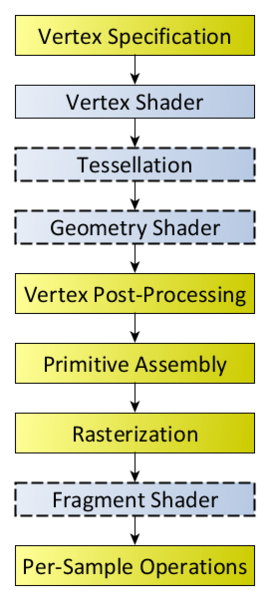
\includegraphics[width=0.2\textwidth,keepaspectratio]{renderPipeline.png}
    \caption[Programmierbare Render-Pipeline]{Programmierbare Render-Pipeline\protect\footnotemark}
    \label{renderPipeline}
\end{wrapfigure}
\footnotetext{\url{https://www.khronos.org/opengl/wiki/Rendering_Pipeline_Overview}}

Des Weiteren ist die Architektur der programmierbaren Render-Pipeline erwähnenswert, welche in Abbildung \ref{renderPipeline} dargestellt ist. Dabei sind programmierbare Abschnitte in blau eingefärbt und optionale Abschnitte mit gestrichelter Linie umrandet. Dies ist der modernere und empfohlene Weg die API zu nutzen und steht ab der OpenGL Version 3.2 zur Verfügung, was heutzutage auf fast jedem System verfügbar ist. Die Shader an sich werden dabei einer Sprache namens GLSL geschrieben und es gibt 2 Wege, Daten an einen Shader zu übergeben. Der erste ist die Übergabe als Vertex-Attribut, bei dem jedem Vertex beliebig viele andere Daten, zum Beispiel Normalenvektoren, zugeordnet werden können. Diese sind in der Regel fest pro Modell definiert und können zur Laufzeit nicht geändert werden. Dagegen sind Uniform Werte unabhängig von einzelnen Vertices und können pro Render-Aufruf geändert werden.

Die einzelnen definierten Vertices werden als erstes vom Vertex-Shader bearbeitet. Dieser transformiert den Vertex in der Regel an Hand von verschiedenen Parametern (Kameraposition, Position des Objektes, Perspektive). Auch andere Berechnungen, welche pro Vertex ausgeführt werden müssen, können hier durchgeführt werden. Anschließend werden die Vertices, welche schlussendlich Polygone (Primitives) bilden, in der Tessellation Stufe in kleinere Polygone zerlegt. Damit können zum Beispiel saubere Kurven erzeugt werden, da lange Kanten so häufiger durchbrochen werden. Anschließend gibt es einen optionalen Geometry-Shader, der aus dem Polygon beliebig viele andere Polygone erzeugen kann. Dies ist für die prozedurale Erstellung von Objekten, zum Beispiel für die Darstellung von Gras, sehr hilfreich. In der Vertex Post-Processing Stufe werden die Vertices mit Hilfe des Viewports in das Koordinatensystem des Ausgabefensters transformiert und Vertices welche außerhalb davon liegen oder vom Betrachter weg zeigen (Backface Culling) werden verworfen. In der Rasterization Stufe werden einzelnen Vertices jetzt sogenannte Fragments zugeordnet, aus denen dann die Werte für die Pixel zusammengestellt werden. Ein Pixel kann dabei auch aus mehreren Fragments bestehen. Anschließend wird der Fragment-Shader pro Fragment einmal ausgeführt, welcher auf Grund verschiedenster Parameter eine Farbe für dieses Fragment berechnen muss. In der Per-Sample Operations Stufe kommen verschiedene Techniken zum Einsatz, welche pro Pixel ausgeführt werden. Hier wird zum Beispiel geprüft ob der Pixel einer anderen Anwendung gehört (also ein anderes Fenster das eigene Fenster überlappt), ob der Pixel überhaupt innerhalb des Fensters ist (Scissor Test) oder ob der Pixel von einem anderen Pixel verdeckt ist (Depth Test). Die fertigen Pixel werden dann in einen Framebuffer geschrieben, welcher vom Betriebssystem verwaltet wird und welcher dann vom Monitor angezeigt wird.

Wichtig für das weitere Verständnis ist auch noch das OpenGL interne Koordinatensystem, welches sich vom bekannten mathematischen, kartesischen Koordinatensystem unterschiedet. Die positive x-Achse zeigt bei OpenGL nach rechts, die positive y-Achse nach oben und die positive z-Achse zeigt aus dem Bildschirm nach außen. Der Koordinatenursprung ist dabei immer im Mittelpunkt des Bildschirms um unabhängig von der Bildschirmgröße zu sein. Auch gibt es eine vereinfachte Version des OpenGL Standards namens OpenGL ES, die einen deutlich kompakteren Umfang bietet und unter anderem die Geometry-Shader nicht unterstützt. Implementierungen dieser Version stehen unter dem Namen WebGL auch in allen neueren Browsern zur Verfügung.

\section{Datenreduzierung}\label{datenreduzierung}

\subsection{Datenmenge}\label{datenmenge}
Der beschriebene MOLA-Datensatz besitzt eine Breite von 46080 Pixeln und eine Höhe von 23040 Pixeln. Jeder Pixel ist dabei 16 Bit groß, sodass die Rohdaten an sich eine Größe von 1,98 GB besitzen\cite{molaDataExtended}. Um daraus ein 3D-Modell zu erstellen, müssen neben den Höhenwerten natürlich auch die x- und z-Position erfasst werden, welche sich aus dem Rasterformat der Daten errechnen lassen. Erschwerend hinzu kommt, dass der kleinste numerische Datentyp in GLSL 32 Bit groß ist\cite[Abschnitt 4.1]{glslSpec} und sich die Höhendaten so nicht effizient speichern lassen. Eine entsprechende Erweiterung (\textit{extension}) von GLSL um 16 Bit Typen mit dem Namen EXT\_shader\_16bit\_storage existiert, befindet sich allerdings erst in der Entwurfsphase und kann daher nicht genutzt werden. Die reinen Vertex-Daten besitzen also eine Größe von 11,88 GB. Weitere Daten pro Vertex (zum Beispiel Normalenvektoren) werden für dieses Projekt nicht benötigt. Allerdings können diese Vertex-Daten in dieser Form nicht an OpenGL übergeben werden, da erst Polygone (OpenGL Primitives) daraus erstellt werden müssen. Im einfachsten Fall sind dies für ein Rastermodell natürlich Vierecke (GL\_QUAD), diese Form ist allerdings veraltet und sollten nicht mehr benutzt werden. Stattdessen müssen die Vertex-Daten  Dreiecke (GL\_TRIANGLE) beschreiben. Da in einem Rastermodell aus Dreiecken natürlich ein Vertex 6 mal wiederholt werden müsste, gibt es eine effizientere Beschreibung der Polygone: Indexierung. Dabei wird ein Array an OpenGL übergeben, welche die Reihenfolge der Vertices als deren Position im ursprünglichen Vertex-Array kodiert (siehe Abbildung \ref{indexing}). 

\begin{figure}[H]
  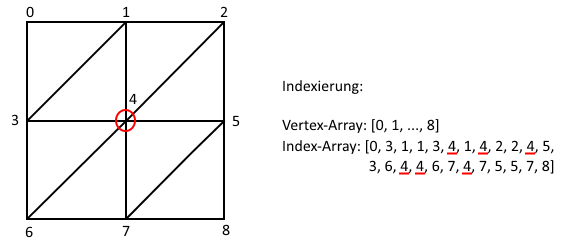
\includegraphics{indexing.png}
  \caption{Indexierung eines Raster-Modells}
  \label{indexing}
\end{figure}

Durch diese Technik wird das Wiederholen eines Vertex verhindert, allerdings ist auch hier ein Speicherverbrauch zu berechnen. Der Index entspricht dabei einer Größe von 32 Bit und die Anzahl lässt sich mit folgender Formel berechnen: \[Anzahl = 6 * (H\ddot{o}he - 1) * (Breite - 1) = 6.369.684.486\]. Dadurch werden weitere 23,73 GB benötigt, wodurch der Gesamtspeicherverbrauch auf 35,61 GB steigt. Da dies, auch ohne nicht-funktionale Anforderungen definiert zu haben, nicht in einen durchschnittlichen Grafikspeicher passt, sind Maßnahmen zur Reduzierung der Daten zwingend erforderlich.

\subsection{Verlustfrei}
Das Durchführen von verlustfreien Methoden zur Reduzierung der Datenmenge ist natürlich immer den verlustbehafteten Methoden vorzuziehen, da eine Ansicht mit möglichst großem Detailgrad ein Kernaspekt dieser Arbeit darstellt. Die einfachste Möglichkeit, ist die Entfernung von Redundanzen. Diese können auf Grund des Rasterformats der Daten vorhanden sein, da die Abstände zwischen den Datenpixeln laut Definition einem festen Wert entsprechen müssen. Die hohe horizontale Datenauflösung von 463 m bei einer natürlichen Topographie führt zu der statistischen Annahme, dass dabei Redundanzen auftreten. Hier stellt sich die Frage, was eigentlich eine Redundanz im Kontext von 2D Höhenwerten ist. Ein Auffinden von gleichen Werten in einem 3x3 Raster ist der einfachste Fall. Wichtig hierbei ist, dass nicht etwa ein einfaches Wiederholen von Werten bereits eine Redundanz ist, da auch das Darstellen einer flachen Ebene eine wichtige Information ist. Allerdings können Redundanzen auch bei einer geneigten Ebene auftreten, bei der sich benachbarte Höhenwerte unterscheiden. Der generelle Fall zur Beschreibung ist das Vorhandensein einer linearen Abhängigkeit zwischen Werten in \textbf{allen} Spalten und Reihen eines mindestens 3x3 großen Rasters\cite{topoDataReduction}. Wichtig hierbei ist, dass immer der 2D Kontext beachtet werden muss. Es können sich beliebig viele Werte in einer Reihe oder Spalte wiederholen, ohne das dies eine Redundanz darstellt, wenn auch nur eine Spalte oder Reihe im Raster diese lineare Abhängigkeit nicht aufweist. Um das Vorhandensein von Redundanzen im MOLA Datensatz zu beweisen, wurde ein Script erstellt, welches im Abschnitt \ref{redundanzberechnung} genauer beschrieben ist. Dies zeigt, dass insgesamt 68.264.527 Datenpixel redundant sind, was einem Prozentsatz von 6,43 \% entspricht. Dabei existieren 8.708.542 redundante Teilraster, das größte von ihnen besitzt immerhin eine Fläche von 277.922 km².

Eine andere Möglichkeit eine verlustfreie Reduktion zu erreichen, ist die Daten zu entfernen, die vom Benutzer nicht gesehen werden können. Das betrifft explizit nicht den Punkt, dass Unterschiede auf Grund der Physiologie des menschlichen Auges nicht wahrgenommen werden können, da dies trotzdem einem theoretischen Informationsverlust entspricht. Dabei kommen in der Computergrafik bekannte Techniken zum Einsatz, welche sich nicht auf digitale Geländemodelle beschränken. Zum einen können Daten entfernt werden, die außerhalb des Sichtbereichs der virtuellen Kamera (Frustum) liegen. Dieses \textit{frustum culling} sorgt damit für ein Anstieg der Reduktion bei ansteigendem Zoomfaktor, da dabei immer mehr Teile des Planeten aus dem Sichtbereich verschwinden. Dies ist sehr vorteilhaft, da mit ansteigender Zoomstufe natürlich der Detailgrad und somit auch die Datenmenge ansteigen muss. Eine andere Technik bietet sich an, da bei einem Globus natürlich immer mehr als die Hälfte der Fläche vom Betrachter nicht gesehen werden kann, da sich diese am anderen Ende des Globus befindet. Dieses \textit{occlusion culling} sorgt dafür, dass Daten, welche von anderen verdeckt werden, entfernt werden können. Eine Voraussetzung für beide Techniken ist jedoch die Unterteilung des Welt in kleinere Einheiten. Idealerweise sollte dies für einzelne Polygone oder sogar Vertices angewendet werden, allerdings sind die Berechnungen zu aufwendig um sie pro Frame für alle Vertices durchzuführen. Stattdessen muss hier ein Kompromiss aus Rechenkomplexität und Reduktionsfaktor gefunden werden und es muss akzeptiert werden, dass der gesamte Abschnitte (engl. tile) beibehalten werden muss, selbst wenn nur ein einzelner Vertex durch die Verfahren als sichtbar identifiziert wird. Neben der Datenreduktion helfen diese Verfahren auch bei der Rendering-Performance. Wie beschrieben wird die gesamte Render-Pipeline durchlaufen, inklusive der Ausführung von Vertex- und Fragment-Shader, bevor einzelne Pixel, welche verdeckt werden oder außerhalb des Bildschirms liegen, verworfen werden können. Eine Reduktion von über 50\% ist dabei also sehr positiv.

\subsection{Verlustbehaftet}
Das Durchführen von verlustfreien Methoden allein reicht nicht aus, um den Speicherverbrauch auf ein akzeptables Niveau zu senken. Hier kann dann zum Beispiel ausgenutzt werden, dass Unterschiede in den Daten bei hohen Zoomstufen rein physiologisch nicht mehr wahrgenommen werden können. Grundsätzlich gilt bei allen Methoden, die grobe Struktur des Modells beizubehalten. Diese Methoden entstammen dem Teilgebiet der \textit{mesh simplification} und sind in der Regel nicht auf Geländemodelle beschränkt. Hier wird zwischen lokalen und globalen Reduktionsstrategien unterschieden. Die lokalen Strategien gehen dabei in einem iterativen Prozess vor und und vereinfachen das Modell an Hand lokaler Parameter (Vertices, Kanten, Polygone) und die globalen Strategien nutzen das gesamte Modell als Eingabe. Die lokalen Strategien kommen in der Praxis häufiger zum Einsatz, da deren Berechnung weniger kostenaufwending ist. Sie klassifizieren die lokalen Parameter meist nach ihrer Wichtigkeit an Hand einer vordefinierten Kosten- oder Fehler-Funktion, welche angibt, wie stark sich Änderung auf die Korrektheit des Modells auswirkt. Anschließend werden die Elemente meist mit aufsteigenden Kosten entfernt. Die Entfernung kann solange durchgeführt werden, bis entweder ein gewünschter Reduktionsgrad oder bis eine bestimmte Kostengrenze erreicht ist. Außerdem kann der Fehler zum originalen Modell ein Schwellwert darstellen, hier geht dann jedoch die Lokalität verloren, da hier pro Operation das gesamte Modell betrachtet werden muss\cite[Abschnitt 3]{meshSimplSurvey}. Lokale Strategien haben zum einen das Problem, dass sie nicht die gesamte Topologie betrachten und es so bei komplexeren Modellen zu einer starken Änderung kommen kann. Zum anderen helfen sie nicht dabei, die Reduktion besonders gleichmäßig durchzuführen. Es kann durchaus vorkommen, dass anschließend die Auflösung in bestimmten Bereichen die Anforderung überschreitet. Hier kann der Prozess allerdings so beeinflusst werden, dass die Kosten ansteigen, je geringer die Kosten in der Umgebung des Parameters sind.

Zwei bekannte lokale Strategien sind die \textit{vertex decimation} und die \textit{edge contraction}. Bei der \textit{vertex decimation} werden Vertices klassifiziert und anschließend entfernt. Anschließend muss eine Tesselation stattfinden, bei der die Kanten des entfernten Vertex auf umliegende Vertices verteilt werden. Dabei wird neben der Anzahl der Vertices auch die Anzahl der Polygone reduziert, wenn Kanten sich überlagern und zu einem Polygon ohne Fläche führen\cite[Abschnitt 3.1]{meshSimplSurvey}. Im Kontext von Geländemodelle sollen vor allem die Höheninformationen nicht verloren gehen, die Anstiege (engl. slopes) zwischen einzelnen Werten dürfen sich dabei möglichst wenig ändern. Die Entfernung von Werten in horizontaler Richtung spielt dort dabei keine Rolle, solange die Rechteckstruktur des gesamten Modells beibehalten wird, was bereits durch die Nichtentfernung der Eckpunkte erreicht wird. Eine bekannte Kostenfunktion klassifiziert Vertices danach, wie stark sich der Flächeninhalt des umliegenden 3x3 Rechtecks ändert, sollte der betrachtete Vertex aus der Mitte entfernt werden\cite{topoDataReduction}. Die \textit{edge contraction} Strategie, oft auch oft \textit{edge collapse} genannt, entfernt dagegen Kanten und führt die benachbarten Vertices zu einem neuen Vertex in der Mitte der Kante zusammen. Hier existieren verschieden, unterschiedlich komplexe Kostenfunktionen\cite[Abschnitt 3.2]{meshSimplSurvey}. Eine einfache Funktion klassifiziert die Kanten nach ihrer Länge, da so möglichst kleine Polygone entfernt werden und der Fehler im Durchschnitt relativ gering ist. Diese Strategie kann besonders gut auf Höhenmodelle angewandt werden, da die Kantenlänge in einem gleichmäßigem Rastermodell mit dem Anstieg proportional ansteigt.

Zwei bekannte globale Strategien sind das \textit{vertex clustering} und die \textit{shape approximation}. Beim \textit{vertex clustering} werden die Vertices danach gewichtet, wie wahrnehmbar sie im Gesamtmodell sind. Zum einen spielt dort eine Rolle, wie groß die Polygone um den Vertex sind und welche Krümmung die umliegende Region aufweist. Anschließend wird ein dreidimensionales Gitter über das Modell gelegt und in jeder Zelle wird nur der Vertex beibehalten, der das größte Gewicht beinhaltet. Durch eine Anpassung der Gittergröße kann leicht die Reduktionsgröße angepasst werden. Außerdem führt es zu einer sehr gleichmäßigen Reduktion, allerdings wird die originale Struktur meist nur sehr schlecht abgebildet\cite[Abschnitt 4.1]{meshSimplSurvey}. Bei der \textit{shape approximation} wird das Modell kleinere Regionen zerlegt, die durch ein möglichst einfaches Polygon approximiert werden. Anschließend werden die Vertices aus dem originalen Modell beibehalten, die mit den Vertices der Approximationen übereinstimmen. Durch die maximale Größe der Teilregionen kann dabei der Reduktionsfaktor beeinflusst werden. Da die Polygone nicht in ihrer Form begrenzt sind führt dieses Verfahren zu geringeren Fehlern, allerdings ist die Unterteilung in passende Regionen ein Problem für sich\cite[Abschnitt 4.2]{meshSimplSurvey}. Ein ähnliches Verfahren namens \textit{adaptive subdivision} versucht auch das Modell möglichst gut zu approximieren. Allerdings geht es den umgekehrten Weg und zerlegt ein einfaches Basismodell, was über das originale Modell gelegt wird, in immer kleiner werdende Abschnitte, die sich an das Modell anpassen. Es nutzt dabei meist nur reguläre Polygone und erreicht so nicht die Komplexität der \textit{shape approximation} und bewertet auch nicht die Struktur des originalen Modells wie beim \textit{vertex clustering}\cite[Abschnitt 4.1.2]{meshSimplOverview}.

Für dieses Projekt soll nur ein einfaches Verfahren zum Einsatz kommen, dass die Struktur nicht betrachtet und einzelne Vertices auch nicht bewertet. Es geht mit einer festen Schrittweite (engl. stride) über die Daten und verwirft alle nicht betrachteten Werte. Dies wird häufig als systematische Reduktion oder als \textit{sampling}\cite[Abschnitt 4.1.3]{meshSimplOverview} bezeichnet. Dies kann nur im Kontext von Geländemodellen zum Einsatz kommen, da hier die Unterschiede zwischen den einzelnen Datenpunkten sehr gering sind. Die Datengrundlage sind natürliche Daten und extreme Schwankungen in der Höhe sind somit nahezu ausgeschlossen. Selbst wichtige Höhenfeatures wie Berge strecken sich über mehrere Kilometer, was bei einer so hohen Datenauflösung selbst bei einer aggressiven Reduktion zu einem sehr geringen Fehler führen sollte. Die größten Vorteile dieses Ansatz ist seine geringe Komplexität und der Fakt, dass die Punkte gleichmäßig entfernt werden. Bei allen anderen Verfahren muss mit einem fertigem 3D Modell gearbeitet werden, da die Position der Höhenwerte codiert werden muss. Die systematische Reduktion kann dagegen auf die Originaldaten angewandt werden, da sich die Position weiterhin aus dem Index berechnen lässt. Ausschließlich die Abstände zwischen den Werten hat sich verändert.

Alle Ansätze generieren mit diesen Methoden in der Regel mehrere Modelle mit unterschiedlichen Auflösungen (\textit{level of detail}), welche zur Laufzeit ausgewählt werden, je nachdem wie weit der Betrachter von dem Modell entfernt ist oder in welche Winkel er dieses betrachtet. Auch der beim Benutzer verfügbare Speicher kann ein Auswahlgrund für die richtige Auflösung sein. Ob eine Reduktion zur Laufzeit bei einem so einfachen Verfahren ausreicht, muss evaluiert werden. Der Nachteil bei der Generierung von mehreren Modellen ist natürlich der große Speicherverbrauch, selbst wenn diese Modelle meist nicht im Arbeitsspeicher gehalten werden.

\subsection{Alternative Verfahren}
Neben den hier beschriebenen Verfahren gibt es Möglichkeiten, die Datenenge durch spezielle Verfahren zu senken. Eine bekannte Möglichkeit ist es, die Daten gar nicht als vollständiges 3D Modell zu interpretieren, sondern dies dem Benutzer nur vorzuspielen. Hierbei wird aus den Daten ein Bild erzeugt, welches als Textur auf ein stark vereinfachtes Modell gelegt werden kann\cite[Abschnitt 5.1]{outOfCore}. Die Textur hat dabei natürlich eine deutlich geringe Größe als das ursprüngliche Modell. Dieses vereinfachte Modell kann dann je nach Anforderung mit den echten Daten verbessert werden, wobei die Textur weiterhin auf der höchsten Auflösung bleibt. Die Generierung der Textur kann dabei einmalig oder zur Laufzeit in bestimmten Zeitabschnitten erfolgen, wodurch die Darstellung sich an Änderungen anpassen kann. Diese Darstellung kann weiterhin durch vorberechnete Licht- und Schattentexturen verbessert werden, da somit Tiefen simuliert werden können. Ein Problem dieses Ansatzes ist unter anderem, dass die echte Geometrie verloren geht und Prozesse wie die Simulation von physikalischen Effekten nicht mehr durchgeführt werden können. Außerdem ist die maximale Größe von Texturen im Gegensatz zur Größe von Modellen durch die OpenGL Implementation definiert (GL\_MAX\_TEXTURE\_SIZE).

Ein etwas anderer Ansatz ist die Generierung des Modells auf eine effizientere Weise. Anstatt des klassischen Rasterfromats, bei denen selbst nach der Redundanzentfernung, die Gitterstruktur vorgeschrieben ist, können sogenannte \textit{triangulated irregular networks} (TINs) verwendet werden. Bei dieser vektorbasierten Struktur können die Messpunkte in einer irregulären Struktur vorliegen. Dabei müssen die Positionsdaten natürlich mit den Höhenwerten zusammen codiert werden, da sie sich nicht mehr aus der Struktur berechnen lassen. Sie ist die effizienteste Form der Darstellung, da sie sie Oberfläche mit der minimalsten Anzahl an Punkten abbildet und fast ohne Konvertierung als 3D Modell genutzt werden kann. Die Erstellung solcher TINs erfordert jedoch relativ komplexe Algorithmen und kann aus einem Rasterformat nur mit einem bestimmtem Fehler durchgeführt werden\cite{tinAlgo}.

Ein weiterer Ansatz ist es, die Datenmenge beizubehalten und den gesamten Rendervorgang auf externen Rechnern durchzuführen. Diese Technik wird auch oft als \textit{out-of-core}-Rendering bezeichnet\cite[Abschnitt 3]{outOfCore}. Diese externe Rechner besitzen dann deutlich bessere Hardware und können so die Limitierung der Benutzerhardware umgehen. Auch ist es möglich, das Rendering auf einen ganzen Cluster aus Rechnern aufzuteilen.  Der Client sendet dabei alle Parameter an den externen Server, welche den Rendervorgang beeinflussen können. Dazu zählen in der Regel alle Benutzeraktionen und Konfigurationsänderungen. Aber auch clientspezifische Dinge wie die Bildschirm-Auflösung müssen bekannt sein. Der Server sendet das fertige Ergebnis als Bild in der passenden Auflösung zurück und dieser updated dann nur seine lokale Ansicht, was weder Speicher noch Hardwareressourcen benötigt. Hier ist vor allem die Framerate ein störendes Problem, da ein Senden über ein Netzwerk durch sein Durchsatz begrenzt ist. Auch existiert dank des Netzwerks eine spürbare Latenz. Die Komplexität der Implementation ist auch nicht zu vernachlässigen, da insbesondere bei der Synchronisation zwischen Server und Client einiges schief gehen kann.

\subsection{Redundanzentfernung}\label{redundanzberechnung}
Bevor ein geeigneter Algorithmus gefunden werden kann, müssen einige Probleme mit der Entfernung von Redundanzen besprochen werden. Zum einen besteht das Problem, die gefundenen Lücken in einem Datenformat darzustellen. Normalerweise besteht immer der gleiche Abstand zwischen zwei benachbarten Datenpunkte, wenn jetzt einfach Vertices entfernt werden, dann ändern sich die Abstände und dies muss irgendwie kodiert werden. Eine Möglichkeit dies zu umgehen, ist die Entfernung zur Laufzeit durchzuführen und direkt bei der Erstellung redundante Vertices zu erkennen. Da der hier verwendete Algorithmus allerdings sehr kostenaufwendig ist, wurde dieser Ansatz verworfen. Stattdessen werden die Lücken durch vordefinierte Werte kodiert, die nicht in den originalen Daten vorhanden sind. Im konkreten Fall wurde der kleinstmögliche 16 Bit Wert gewählt.

Zum anderen besteht das Problem der Indexierung des Modells. In einem reinen Raster-Modell lassen sich die Indices trivial berechnen, da sie immer einem gleichmäßigem Muster folgen. Jetzt existieren natürlich Lücken in den Vertex-Daten und eine neues Polygon Netz muss gefunden werden. Ein Problem dabei ist, dass benachbarte Vertices sich mit den Rändern der Lücken verbinden müssen (siehe Abbildung x). Auch wenn die Ränder also redundante Daten aufweisen, müssen sie für die Erzeugung eines korrekt aussehenden Modells zugelassen werden. Anstatt also nur die Eckpunkte zu erhalten, müssen auch alle Ränder der Redundanzen erhalten bleiben, was den Prozentsatz der redundanten Vertices auf 1,87 \% drückt. Für die Berechnung der Indices wurde folgende Formel genutzt: TODO.

Wie beschrieben, ist die Unterteilung des Gesamtmodells in Abschnitte ein zentraler Aspekt der Anwendung um das \textit{frustum-} und \textit{occlusion culling} durchführen zu können. Die führt aber zu einer weiteren Einschränkung bei der Entfernung von Redundanzen, die über Abschnittsgrenzen hinaus gehen würden. Die müssen an den Rändern der Abschnitte definiert sein, um sich mit benachbarten Abschnitten verbinden zu können. Auch sollen per Design Abschnitte keinen Zugriff auf Vertex-Daten anderer Abschnitte erhalten (schon allein um Daten nicht unnötig im RAM zu halten). Dies führt dazu, dass der Algorithmus zusätzlich redundante Teilraster an den Abschnittsgrenzen trennen muss. Dies verringert den Prozentsatz allerdings nur minimal auf 1,86 \%.

Nachdem nun Anforderungen an den Algorithmus definiert wurden, muss das Problem der hohen Komplexität angegangen werden. Die optimale Lösung ist durch die größtmögliche Entfernung von Vertices definiert, was auch durch eine möglichst große Summe des Flächeninhalts aller Teilraster beschrieben werden kann. Das Problem ist, dass während der Laufzeit nicht sichtbar ist, welche Konfiguration der Raster zur größtmöglichen Fläche führt. Es kann durchaus sein, dass in einem Teilschritt ein kleineres Raster gebildet werden muss, damit übrig gebliebene Vertices Teil eines deutlich größeren Rasters werden. Das diesem Problem am nächsten stehende bekannte Problem aus der Informatik ist das Problem des \textit{rectangle packing}, einer 2D Variation des Rucksack-Problems, welches der Komplexitätsklasse NP-Vollständig zugerechnet wird. Die Überprüfung ob eine Lösung optimal ist, erfordert dabei das Überprüfen aller anderen Lösungen, was eine exponentielle Zeit benötigt. Allerdings sind im konkreten Fall einige Einschränkungen vorhanden, die die Komplexität verringern. Zum einen können die Rechtecke nicht an jede Stelle gepackt werden, sondern nur in den Flächen, die als Redundanzen in Frage kommen. Zum anderen ist die Mindestgröße eines Rechtecks 3x3, sodass sich die Anzahl der Möglichkeiten um den Faktor 9 verringert. Unter der Annahme, dass die aktuelle, nicht optimale Berechnung die Anzahl der Gesamtredundanzen mit ungefähr 2 \% widerspiegelt, ist die Komplexität: \[O(n) = O(1.061.683.200) = 2^{n / 9 * 2 / 100} = 7.32 * 10^{710.218}\]

Als machbare Alternative wurde hier ein Algorithmus aus der Klasse der greedy Algorithmen entwickelt. Dabei wird in jedem Teilschritt des Algorithmus immer die aktuell beste Lösung, also das größte Teilraster, gewählt. Die gefundene Lösung ist damit zwar nicht unbedingt optimal, aber es wird ein lokales Minimum erreicht. Der größte Vorteil dabei ist, das die Lösung mit fast linearer Komplexität gefunden werden kann. Die Komplexität ist leicht erhöht, da pro Wert immer eine nicht bestimmbare Anzahl an nachfolgenden Werten überprüft werden muss. Diese können aber potentiell bei nachfolgenden Iterationen übersprungen werden, falls sie als redundant eingestuft wurden. Der Algorithmus (siehe Algorithmus \ref{redundanz_algorithmus}) iteriert über alle Werte und sucht für jeden nicht besuchten Datenpunkt alle nachfolgenden horizontalen und vertikalen linearen Abhängigkeiten. Dabei werden jeweils die Breiten und Längen dieser Abhängigkeiten zurückgeliefert und auch alle Alternativen in Betracht gezogen. Es können zum Beispiel bei den Reihen jeweils 3 Reihen eine Breitenlänge von 4 haben oder 5 Reihen eine Breitenlänge von 3. Beides kann zum größtmöglichen Raster führen. Dies wird auch für die Spalten durchgeführt und die größtmögliche Überschneidung aus Spalten und Reihen wird als redundant markiert, solange sie die Mindestgröße von 3x3 erreicht hat.

\begin{algorithm}[H]
\begin{algorithmic}
\caption{Redundanzentfernung}
\label{redundanz_algorithmus}
\Procedure{findRedundancies}{data, replacement, chunkSize}
    \ForAll{x, z \textbf{in} data}
        \If{Wert an Stelle x, z noch nicht besucht}
            \State rows = Finde alle Abhängigkeiten in den Reihen ab x, z (checkRows)
            \State columns = Finde alle Abhängigkeiten in der Spalten ab x, z
            \State raster = Finde das Raster mit dem größten Flächeninhalt in rows, columns
            \If{raster hat Mindestgröße 3x3}
                \State Ersetze alle Werte in raster, die nicht Kanten sind, mit replacement
                \State Markiere alle Werte in raster als besucht
            \EndIf
        \EndIf     
    \EndFor
\EndProcedure
\Procedure{checkRows}{data, currentX, currentZ, chunkSize}
    \ForAll{z von currentZ bis Ende der Reihen oder Ende des Chunks}
        \State difference = data[z][x] - data[z][x + 1]
        \ForAll{x von currentX bis Ende der Spalte oder Ende des Chunks}
            \If{nächste Differenz == difference}
                \State Inkrementiere aktuelle Breite
            \ElsIf{aktuelle Breite $<$ 3}
                \State\Return alle Breitenlängen und deren Reihen
            \ElsIf{aktuelle Breite $<$ letzte Breite}
                \State Speichere Breitenlänge und Reihe
                \State letzte Breite = aktuelle Breite
                \State Weiter mit nächster Reihe
            \Else
                \State Weiter mit nächster Reihe
            \EndIf
        \EndFor
    \EndFor
    \State\Return alle Breitenlängen und deren Reihen
\EndProcedure
\end{algorithmic}
\end{algorithm}